\subsection{EP energy: a primal-dual story}
\label{sec:chap2_ep_energy}

EP has been criticised for not having convergence guarantees and instead being a heuristic for posterior approximation. On the other hand, it has been shown to have superior performance compared to VI on a variety of tasks, e.g.~Gaussian Process classification \citep{kuss:gpep2005}. To understand these seemingly contradicting observations, here we provide an energy minimisation view of EP,\footnote{material based on my NIPS 2016 approximate inference workshop abstract, see publication page.} and discuss why EP could potentially lead to better approximations, and why it is difficult to prove the convergence of EP. Similar derivations are also available in \citet{yedidia:bethe2001, heskes:ep2002, minka:divergence2005, opper:ec2005, wainwright:graphical2008}, and some extensions to handling latent variable models are provided in appendix \ref{sec:appendix_relaxation}.

To streamline the notation, we consider approximating the intractable posterior $p(\mparam|\mathcal{D}) = \frac{1}{Z} p_0(\mparam) \prod_{n=1}^N p(\bm{x}_n|\mparam)$ as a running example. In this case we denote $\tilde{f}_n(\mparam) = p(\bm{x}_n|\mparam)$ and leave the prior $p_0(\mparam)$ as it is. Using this notation we again write down the objective function of Variational inference (VI) called the \emph{variational free energy} (VFE) \citep{jordan:vi1999, beal:vi2003}:
\begin{equation}
\min_{q \in \mathcal{Q}} \mathrm{KL}[q||p] \Leftrightarrow \min_{q \in \mathcal{Q}} \mathcal{F}_{\text{VFE}}(q) = \mathbb{E}_{q} \left[ \log q(\mparam) - \log p_0(\mparam) - \sum_{n=1}^N \log \tilde{f}_n(\mparam) \right].
\label{eq:ep_section_vfe}
\end{equation}

\subsubsection{From VFE to Bethe Free Energy}
\label{sec:vfe_to_bethe}

First we make use of the additivity of logarithm to rewrite an equivalent optimisation problem (recall that $\mathcal{P}$ is the space of all probability distributions):
\begin{equation}
\begin{aligned}
\min_{q \in \mathcal{Q}} \mathcal{F}_{\text{VFE}}(q)
&= \min_{q \in \mathcal{Q}} \mathrm{KL}[q||p_0] - \sum_n \mathbb{E}_{q} \left[ \log \frac{p_0(\mparam) \tilde{f}_n(\mparam)}{q(\mparam)} \right] - N \mathrm{KL}[q || p_0] \\
& = \min_{ q \in \mathcal{Q}, \{ \tilde{p}_n \in \mathcal{P} \} } (1 - N) \mathrm{KL}[q||p_0] - \sum_n \mathbb{E}_{\tilde{p}_n} \left[ \log \frac{p_0(\mparam) \tilde{f}_n(\mparam)}{\tilde{p}_n(\mparam)} \right] \\ 
& \quad \quad \quad \quad \text{ subject to } \tilde{p}_n = q, \forall n. 
\end{aligned}
\label{eq:vi_constrained}
\end{equation}
%
Here in the first line we added $N$ copies of $\mathrm{KL}[q || p_0]$ to the VFE and subtracted the same, and in the second line we \emph{decoupled} the tilted distribution $\tilde{p}_n$ from $q$ by introducing equality constraints. This means the above optimisation has the same fixed points as minimising VFE. The constraints can be \emph{relaxed} to matching all the moments $\mathbb{E}_{\tilde{p}_n}[\mparam^{k}] = \mathbb{E}_q[\mparam^k]$ for $k \in \mathbb{N}$,\footnote{Having the same moments for $p$ and $q$ does not imply having the same \emph{moment generating function}.} and a further crude relaxation suggests moment matching just for the first $K$ moments\footnote{The zeroth moment matching constraint is replaced by the constraint that $\tilde{p}_n$ integrates to 1.}
$\mathbb{E}_{\tilde{p}_n}[\mparam^{k}] = \mathbb{E}_q[\mparam^k], k = 1, 2, ..., K$.
%
In the following we use a vectorial function $\bm{\Phi}(\mparam)$ to summarise these constraints as $\mathbb{E}_{\tilde{p}_n}[\bm{\Phi}] = \mathbb{E}_q[\bm{\Phi}]$, where as an example for Gaussian EP: $\bm{\Phi}(\mparam) = [\mparam, \mparam \mparam^T]$. In general $\bm{\Phi}$ can contain any polynomial terms or other basis functions. This relaxation returns the following constrained optimisation problem:
%
\begin{equation}
\begin{aligned}
 \min_{ q \in \mathcal{Q}, \{ \tilde{p}_n \in \mathcal{P} \} } \mathcal{F}_{\text{Bethe}}( \{ \tilde{p}_n \}, q) \quad \text{subject to } \mathbb{E}_{\tilde{p}_n}[\bm{\Phi}] = \mathbb{E}_q[\bm{\Phi}], \forall n, \\
\mathcal{F}_{\text{Bethe}}( \{ \tilde{p}_n \}, q) =  (1 - N) \mathrm{KL}[q||p_0] - \sum_n \mathbb{E}_{\tilde{p}_n} \left[ \log \frac{p_0(\mparam) \tilde{f}_n(\mparam)}{\tilde{p}_n(\mparam)} \right].
\end{aligned}
\label{eq:bethe}
\end{equation}
$\mathcal{F}_{\text{Bethe}}( \{ \tilde{p}_n \}, q)$ is the \emph{Bethe free energy} \citep{bethe:energy1935, yedidia:bethe2001} that is usually presented in the context of probabilistic graphical models and belief propagation. Below we show how to derive its dual form that is usually discussed in EP literature \citep{minka:ep_energy2001, opper:ec2005, seeger:ep2005}. 

\vspace{1em}
\begin{tcolorbox}
\textbf{Remark} (Tom Minka's original note)\textbf{.}
\cite{minka:ep_energy2001} formulated (\ref{eq:bethe}) as a minimax problem ($\min_{\{\tilde{p}_n \}} \max_{q}$) instead which seems questionable to me.  First (\ref{eq:bethe}) relaxes the constraints in (\ref{eq:vi_constrained}), meaning both should have the same optimisation direction. Then since (\ref{eq:vi_constrained}) just decouples VFE (\ref{eq:ep_section_vfe}) with equality constraints, it should be a pure minimisation and has the same stationary points. For graphical models the Bethe free energy optimisation problem is formulated as a pure minimisation problem like above (\ref{eq:bethe}), e.g.~in \cite{heskes:bp_fixed_point2002, wainwright:graphical2008} but also interestingly in pages 3-4 of \cite{minka:ep_energy2001}. On the other hand, Minka's derivation of the dual energy differs from solving the Lagrangian and does not require the minimax assumption of the primal problem. 
\end{tcolorbox}

\subsubsection{From Bethe to EP: a dual form representation}
\label{sec:ep_fixed_points}
We provide a derivation in a similar way as \cite{heskes:bp_fixed_point2002}, starting from a note on the KL duality\footnote{We include this step in order to connect to the EP energy with optimisation arguments all in the dual space.}
\begin{equation}
 -\mathrm{KL}[q||p_0] = \min_{\bm{\lambda}_{q}(\mparam)} - \mathbb{E}_q[\lambda_q(\mparam)] + \log \mathbb{E}_{p_0} \left[ \exp [\lambda_q(\mparam)] \right],
 \label{eq:kl_duality}
\end{equation}
with $\lambda_q(\mparam)$ a function to be specified later on. This duality is in the same spirit as deriving convex conjugate function for the log partition function of an exponential family distribution (see Proposition \ref{prop:chap2_expfam}), if viewing $p_0(\mparam)$ as the base measure.
The equality is achieved by $q(\mparam) \propto p_0(\mparam) \exp[\lambda_q(\mparam)]$.
%
Substitution into (\ref{eq:bethe}) then yields a transformed energy that we denoted as $\mathcal{F}_{\text{Bethe}}(\{ \tilde{p}_n \}, q, \lambda_q(\mparam))$.
%
\begin{equation}
\begin{aligned}
\mathcal{F}_{\text{Bethe}}(\{ \tilde{p}_n \}, q, \lambda_q(\bm{\theta})) = (1 - N) \mathbb{E}_q[\lambda_q(\bm{\theta})] + (N - 1) \log \mathbb{E}_{p_0} \left[ \exp [\lambda_q(\bm{\theta})] \right] \\
- \sum_n \mathbb{E}_{\tilde{p}_n} \left[ \log \frac{p_0(\bm{\theta}) \tilde{f}_n(\bm{\theta})}{\tilde{p}_n(\bm{\theta})} \right].
\label{eq:bethe_energy_transformed}
\end{aligned}
\end{equation}

%
Denote $\bm{\lambda}_{-n}$ as the Lagrange multiplier for moment matching and $\nu, \nu_n$ for the normalisation constraints of $q$ and $\tilde{p}_n$, respectively. This returns the following Lagrangian
\begin{equation}
\begin{aligned}
 \min_{q, \{ \tilde{p}_n \}, \lambda_q(\bm{\theta}) } \max_{\{ \bm{\lambda}_{-n}, \nu_n, \nu \} } \mathcal{F}_{\text{Bethe}}( \{ \tilde{p}_n \}, q, \lambda_q(\bm{\theta})) + \sum_n \bm{\lambda}_{-n}^{T}(\mathbb{E}_q[\bm{\phi}] - \mathbb{E}_{\tilde{p}_n}[\bm{\phi}]) \\
 + \sum_n \nu_n \left( \int \tilde{p}_n(\bm{\theta}) d\bm{\theta} - 1 \right) + \nu \left( \int q(\bm{\theta}) d\bm{\theta} - 1 \right) .
\end{aligned} 
\label{eq:bethe_lagranrian}
\end{equation}
Solving the fixed points for $\tilde{p}_n$ and $\nu_n$ returns 
$$
\tilde{p}_n(\mparam) = \frac{1}{Z_n} p_0(\mparam)\tilde{f}_n(\mparam) \exp \left[ \bm{\lambda}_{-n}^T \bm{\Phi}(\mparam) \right],
$$
where the normalising constant is $$Z_n = \int p_0(\mparam) \tilde{f}_n(\mparam) \exp \left[ \bm{\lambda}_{-n}^T \bm{\Phi}(\mparam) \right] d \mparam.$$ 
%
Also it is straight-forward to evaluate the fixed point condition for $q$: $$(N - 1) \lambda_q(\mparam) = \sum_n \bm{\lambda}_{-n}^T \bm{\Phi}(\mparam) + \nu.$$
We explicitly specify $\lambda_q(\mparam) = \bm{\lambda}_q^T \bm{\Phi}(\mparam) + \nu$ w.l.o.g., also the constant $\nu$ can be dropped since exponential family distributions are translation invariant to constants.
%
Importantly, substituting $\tilde{p}_n$ back to (\ref{eq:bethe_lagranrian}) and enforcing the fixed point condition for $q$ yields the \emph{EP energy} \citep{minka:ep_energy2001}:
\begin{equation}
\begin{aligned}
\min_{\bm{\lambda}_q} \max_{\{ \bm{\lambda}_{-n} \} } \mathcal{F}_{\text{EP}}(\bm{\lambda}_q, \{ \bm{\lambda}_{-n} \} ) =  (N - 1) \log \mathbb{E}_{p_0} \left[ \exp [\bm{\lambda}_q^T \bm{\Phi}(\mparam)] \right] - \sum_n \log Z_n,\\
 \text{subject to } (N - 1) \bm{\lambda}_q = \sum_n \bm{\lambda}_{-n}.
\end{aligned}
\label{eq:ep_energy}
\end{equation}
Notice now the optimisation problem over $q$ is dropped since (\ref{eq:ep_energy}) does not depend on it. To obtain the approximate posterior back, we make use of the tightness of the KL duality, and define 
$$q(\mparam) = \frac{1}{Z_q} p_0(\mparam) \exp \left[ \bm{\lambda}_q^T \bm{\Phi}(\mparam) \right],  \quad \log Z_q = \log \mathbb{E}_{p_0} \left[ \exp [\bm{\lambda}_q^T \bm{\Phi}(\mparam)] \right].$$
%
The expectation consistent approximate inference (EC) algorithm \citep{opper:ec2005} is a special case with $p_0(\mparam) \propto 1$ and $N = 2$. 

\subsubsection{EP as a fix point iteration method for solving the dual problem}

EP \citep{minka:ep2001} proposes parametrising the (natural parameters of) local approximating factors $f_n \approx \tilde{f}_n$ instead of the approximate posterior $q$, with the goal of $f_n$ capturing the effect of $\tilde{f}_n(\mparam)$ on the exact posterior, by defining $f_n(\mparam) = \exp [\bm{\lambda}_n^T \bm{\Phi}(\mparam)]$, $\bm{\lambda}_n = \bm{\lambda}_q - \bm{\lambda}_{-n}$. Thus by construction the constraint in (\ref{eq:ep_energy}) is automatically satisfied: $\bm{\lambda}_q = \sum_n \bm{\lambda}_n$ and $\bm{\lambda}_{-n} = \sum_{m \neq n} \bm{\lambda}_m$.
%
Then EP runs a fixed point iteration algorithm to find a stationary point for $\{ \bm{\lambda}_n \}_{n=1}^N$. More specifically the gradient of (\ref{eq:ep_energy}) w.r.t.~the local parameter $\bm{\lambda}_n$ is 
\begin{equation}
\nabla_{\bm{\lambda}_n} \mathcal{F}_{\text{EP}} = (N-1) \mathbb{E}_{q} [ \bm{\Phi}(\mparam) ] - \sum_{m \neq n} \mathbb{E}_{\tilde{p}_m} [ \bm{\Phi}(\mparam) ].
\end{equation} 
Zeroing the above gradient for all $\bm{\lambda}_n$ results in the fixed point condition
$$\mathbb{E}_q[\bm{\Phi}(\mparam)] = \mathbb{E}_{\tilde{p}_n}[ \bm{\Phi}(\mparam) ], \quad \forall n,$$
which motivates the moment matching update (\ref{eq:chap2_ep_moment_matching}) in EP.

\subsubsection{A pictorial view on why EP can be better than VI}
Folk wisdom suggests that EP, if it convergences, often provide more accurate approximations to the target distribution when compared with VI. This observation is explained pictorially in Figure \ref{fig:chap2_ep_vi_comparison}. 
%
Recall that both algorithms can be viewed as minimising the Bethe free energy under constraints: for VI the constraints are equality constraints $q = \tilde{p}_n$, whereas EP instead uses moment matching constraints $\mathbb{E}_q[\bm{\Phi}] = \mathbb{E}_{\tilde{p}_n}[\bm{\Phi}]$. In an augmented space $\mathcal{P}^{N+1}$, the search space of VI $\{ (q, \tilde{p}_n): q = \tilde{p}_n, q \in \mathcal{Q} \}$ is contained in the search space of EP $ \{ (q, \tilde{p}_1, ..., \tilde{p}_N): q \in \mathcal{Q}, \mathbb{E}_{\tilde{p}_n}[\bm{\Phi}] = \mathbb{E}_q[\bm{\Phi}] \}$, and can be of much smaller dimensions (e.g.~the green line segment versus the blue region as shown in the Figure \ref{fig:chap2_ep_vi_comparison}). Therefore if EP converges, then it is more likely to find a better minimum compared to VI. Empirical evidence also suggests that constrained Bethe free-energy evaluated at a fixed point is often a better approximation to the (negative log) marginal likelihood.

\begin{figure}
\centering
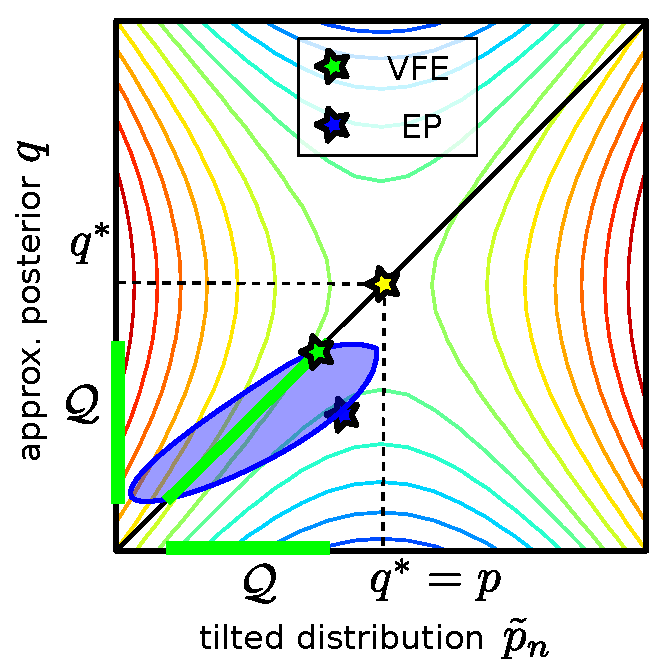
\includegraphics[width=0.4\linewidth]{Chapter2/ep/energy.pdf}
\caption{EP versus VI as constrained energy optimisation problems, visualised by projecting the energy surface from the augmented space $\mathcal{P}^{N+1}$ to $\mathcal{P}^{2}$. Here the slash line across the space represents the subspace $\{ (q, \tilde{p}_n): q = \tilde{p}_n \}$, and the search space for VI (the green segment) is contained in the EP candidate set (the blue region). The stars indicate the optimal solutions returned by the exact (in yellow) and the approximate inference algorithms (green/blue). See main text for details.}
\label{fig:chap2_ep_vi_comparison}
\end{figure}

\subsubsection{Criticisms for EP's iterative update}
%
The above fixed point iteration update has no convergence guarantee, which is one of the drawbacks of EP. The reason is that EP solves the dual problem of constrained Bethe free energy minimisation, and that dual problem turns out to be a minimax optimisation problem with constraints. Indeed, a double-loop algorithm \citep{heskes:ep2002} should be applied to (\ref{eq:ep_energy}) if convergence is required. However in practice such a double-loop method has been shown to be much slower than EP. Also disappointedly, even when the exact posterior is contained in $\mathcal{Q}$, EP is not guaranteed to return it. Similar problems exist for belief propagation when the graph contains many loops, or when the relaxed polytope is not \emph{tight} \citep{wainwright:graphical2008}.

%\hl{Another myth about EP is the choice of using fixed point update instead of gradient descent for the local parameters. Here it should be emphasised that the optimisation aims to find a \emph{saddle point} rather than a local minimum/maximum of the energy function. Since it is a minimisation problem for $\bm{\lambda}_q$ and maximisation problem for $\bm{\lambda}_{-n}$, is is also unclear to determine the optimisation problem for the local parameters $\bm{\lambda}_n$. Finally there exists no proof that the EP energy is upper or lower bounded, i.e. the existence of minimum/maximum is unclear as well. All the above situations make the analysis of gradient descent convergence very difficult.}


\subsubsection{From VFE to power EP}
\label{sec:vfe_to_pep}
We now extend the above approach to power EP \citep{minka:powerep2004} which is a new contribution, although fairly straightforward. This procedure includes one modification to the Bethe free energy. Assume for each factor $\tilde{f}_n$ a power value $\alpha_n \neq 0$ is associated, with $\bm{\alpha} = (\alpha_1, ..., \alpha_N)$ and $\sum_n \frac{1}{\alpha_n} \neq 1$. Then the Bethe free energy with moment matching constraints is modified to:
\begin{equation}
\mathcal{F}_{\bm{\alpha}}(q, \{ \tilde{p}_n \}) = \left( 1 - \sum_n \frac{1}{\alpha_n} \right) \mathrm{KL}[q||p_0] - \sum_{n=1}^N \frac{1}{\alpha_n} \mathbb{E}_{\tilde{p}_n} \left[ \log \frac{p_0(\mparam) \tilde{f}_n(\mparam)^{\alpha_n}}{\tilde{p}_n(\mparam)} \right].
\label{eq:alpha_bethe}
\end{equation}
%
Similar to the derivation of (\ref{eq:vi_constrained}), here we first added and subtracted $(\sum_n \frac{1}{\alpha_n})$ copies of $\mathrm{KL}[q||p_0]$, then decoupled $\tilde{p}_n$ from $q$, and relaxed the equality constraints to moment matching. Calculations following Section \ref{sec:ep_fixed_points} also reveal the change of the fixed point condition for $q$ to $(\sum_n \frac{1}{\alpha_n} - 1) \bm{\lambda}_q = \sum_n \frac{1}{\alpha_n} \bm{\lambda}_{-n}$. Define $q$ as an exponential family distribution with natural parameter $\bm{\lambda}_q$ as before, and $\bm{\lambda}_n = (\bm{\lambda}_q - \bm{\lambda}_{-n}) / \alpha_n$. We arrive at the power EP objective:
\begin{equation}
\left( \sum_n \frac{1}{\alpha_n} - 1 \right) \log Z_q - \sum_n \frac{1}{\alpha_n} \log \int p_0(\mparam) \tilde{f}_n(\mparam)^{\alpha_n} \exp \left[ (\bm{\lambda}_q - \alpha_n \bm{\lambda}_n)^T \bm{\Phi}(\mparam) \right] d \mparam.
\label{eq:pep_energy}
\end{equation}
The iterative process also enforces $\bm{\lambda}_q = \sum_n \bm{\lambda}_n$.  \cite{minka:divergence2005} showed that (\ref{eq:pep_energy}) becomes an upper-bound of $\log Z$ when $\alpha_n > 0$ and $\sum_n \frac{1}{\alpha_n} < 1$. On the other hand, taking $\alpha_n \rightarrow 0, \forall n$ recovers $\mathcal{F}_{\text{VFE}}$ but now the $q$ distribution is restricted to have an exponential family form.